%!TEX root = ../report.tex

% 
% Related work
% 
% (~17pgs)
\section{Related Work}

% começar por dizer como é que está organizada esta secção do trabalho e resumir de uma forma muito geral o que se fala em cada subsecção

This section presents the related work for this project and characterizes the main contributions of past works and how these contributions helped in the development of this project. This section is organized is the main parts: mHealth, mobile security and TrustZone.

The first part focuses on describing the attack surfaces of mHealth apps, the most common threats and their seriousness, present a few publicly available unsecure mHealth apps as well as some compliance recommendations that app developers should follow to avoid unnecessary security risks when handling sensitive health information. The second part of this sections describes the state of the art of mobile security with a particular focus on the Android Operating System and how developers can build secure applications with a trusting \ac{OS} and security mechanisms built upon the application layer. The third part of the related work describes TrustZone, a hardware technology available a most modern \ac{ARM} processors which supports executions of two isolated worlds, a hardware secure world and a normal world. Besides describing the technology this sections also presents previous work developed using TrustZone and who these previous contributions may be helpful in achieving the main goals of this project. 

\subsection{mHealth}

As discussed above, mobile devices are increasing in number at astonishing rates and with this growth the mobile market becomes cheap and accessible. This motivates the shift from mainframe systems located in the facilities of healthcare providers to apps on mobile devices as well as storage in shared could services. This accessibility also motivates the private sector in building more healthcare applications to support both patients and healthcare agents. Thus, the mobile health market is becoming a competitive market and one which is increasingly handling with more sensitive data.

%falar sobre as duas citations abaixo (ler os papers)
Kotz, David \cite{kotz2011threat} defines a threat taxonomy for mHealth. Avancha, Baxi and Kotz \cite{avancha2012privacy} surveyed the literature and developed a privacy framework for mHealth as well as discussed the technologies that could support privacy-sensitive mHealth systems.

% SECURITY CONCERNS MHEALTH ANDROID
% ler os papers citados aqui
He, Dongjing, et al. \cite{he2014security} analyse several mHealth applications available in Android's app store contributing to the understanding of security and privacy risk on the Android platform.

In this paper, three studies were made with the following goals:
\begin{itemize}
	\item \textbf{Study 1: What are the potential attack surfaces?}
	\item \textbf{Study 2: How widespread is the threat?}
	\item \textbf{Study 3: How serious is the threat?}
\end{itemize}

% ler os papers citados aqui
 In the first study 160 apps are analysed to find evidence of threats. From analysing previous literature \cite{zhou2013identity,naveed2014inside,aviv2012practicality,cai2012practicality,chin2011analyzing,fsecure,sevenwaystohangyourselfwithandroid}, seven attack surfaces are determined to be in need of protection. These seven attack surfaces are shown in table \ref{tab:attacksurfaces}.

\begin{table}
	\caption {Description of attack surface (taken from He et al. \cite{he2014security})}
	\label{tab:attacksurfaces}
	\begin{tabular}{|>{\raggedright}p{2cm}|>{\raggedright\arraybackslash}p{10cm}|}
		\hline
		\textbf{Attack Surface}      & \textbf{Description}                                                                                                                    \\ \hline
		Internet            & Sensitive information is sent over the internet with unsecure protocols (e.g. HTTP), misconfigured HTTPS, etc.                 \\ \hline
		Third Party         & Sensitive information is stored in third party servers                                                                         \\ \hline
		Bluetooth           & Sensitive information collected by Bluetooth-enabled health devices can be sniffed or injected                                 \\ \hline
		Logging             & Sensitive information is put into system logs where it is not secured                                                          \\ \hline
		SD Card Storage     & Sensitive information is stored as unencrypted files on SD card, publicly accessible by any other app                          \\ \hline
		Exported Components &  Android app components, intended to be private, are set as exported, making them accessible by other apps                     \\ \hline
		Side Channel        & Sensitive information can be inferred by a malicious app with side channels, e.g. network package size, sequence, timing, etc. \\ \hline
	\end{tabular}
\end{table}
\FloatBarrier

% AQUI ESTOU A DIZER TBM QUE ESCOLHI A APPLICACAO A FAZER POR CAUSA DESTES NUMEROS
In this study the authors also document that the 160 apps studied target two different audiences: 129 (81.65\%) are for patients, 32 (20.25\%) are for healthcare professionals and the remaining 3 (1.90\%) are targeted for both. Most apps targated for patients (60\%) are in the Life Management category followed by apps that manage and synchronize user health information (PHR Management) which occupy nearly half (46.88\%) of these apps. These numbers are a good indicator of what data is handled by most commercial mHealth apps available and motivate the choice made to build a PHR Management app as demo for TrubiZone.

A few examples of vulnerable applications are also revealed during this study. With regard to sending unencrypted information over the Internet, Doctor Online \cite{doctoronline} (patients can talk to doctors online) and Recipes by Ingredients \cite{recipesbyingredients} send unencrypted sensitive information, including the user's email and password, in clear text. With regard to logging sensitive information, the study pinpoints CVS/pharmacy \cite{cvspharmacy}, which logs the prescription refill details from user inputs, including name, email address, store number, and Rx number and also logs user login credentials in a debug log message. A malicious party can use this information to view user profiles, prescription history, which could support medical identity theft and it is even possible to do pharmacy online shopping with user's stored credit card information. Further applications are given as example for exposing sensitive information, Noom Weight Loss Coach \cite{noomwlc} reveals user workout history by exposing its Content Providers to external apps, which means any app can access the exposed Content Providers without declaring any permission. Finally this first study concludes with the example of sleep monitoring apps, such as SnoreClock \cite{snoreclock} and Sleep Talk Recorder \cite{sleeptalk} which store the sleep records of users as unencrypted audio files on external storage. With read permission for the SD card as well as internet permission, a malicious app can read a user's sleep recordings and even send them to remote servers.

In the second study, 27 apps, from the top 1080 free apps from the Medical and Health \& Fitness categories on Google Play, were analysed according to their vulnerabilities. From this analysis three attack surfaces are identified as the most important ones: \emph{Internet}, \emph{Third Party Services} and \emph{Logging}. Only 7 of the 27 apps analysed use the Internet to effectively send medical information over to remote servers. It is important to understand if the information sent over the Internet is protected. To achieve this the authors captured the network traffic and concluded that only 57.1\% (4/7) of these apps use encrypted communication and the remaining 42.9\% (3/7) use unencrypted communication to send sensitive health information. Among the unencrypted contents sent by these 3 apps were emails, usernames and passwords. This study also concludes that 85.7\% (6/7) of these apps are hosted and store the recorded data on third party servers. This is an economical and scalable solution for mobile application, but storing sensitive health records on third party servers can have serious implications, mostly due to app users not being aware that their data is being stored on third party servers and because these users are not able to tell if this data is stored in encrypted is such a way that hosting companies do not have access to this data.

Some health apps use Bluetooth devices to collect personal health information such as heart rate, respiration, pulse oximetry, electrocardiogram (ECG), blood pressure, body weight, body temperature, quality of sleep and exercise activities. Naveed et al. \cite{naveed2014inside} show how a malicious app can stealthily collect user data from an Android device or spoof a device and inject fake data into the original device's app in what is called an \ac{DMB} attack. Ont of the 27 apps analysed in this study connects to external health sensors and uses default PIN code 0000, which makes it vulnerable to the \ac{DMB} attack. Along with the logging, external storage, exported components and the other problems discussed above, which represent the explicit channels used for attacks, side channels can be exploited by a malicious party to infer sensitive information from apps, even when they are well-designed and implemented. This study mentions an example by Zhou et al. \cite{zhou2013identity} where a correlation between network payload size, which is publicly accessible in Android, and the disease condition a user selects on WebMD mobile \cite{webmd}. This problem is mitigated by enforcing limitations on accessing Android public resources by modifying the Android kernel. 

In the third study, another 22 apps, which send information over the Internet, are randomly selected from the same top 1080 apps and used to understand the seriousness of the threat considering the sensitive information sent. The 22 apps are analysed to understand what information is effectively being sent over the Internet and the conclusion is that when used as intended these apps gather, store and transmit a variety of sensitive user data which includes at least personal profiles, health sensor data, lifestyle data, medical information browsing history and third-party app data (e.g. Facebook account information). Figure \ref{fig:sensitivedistribution} shows the distribution of sensitive information in the 22 apps. The consequences of data breaches, information disclosure or tempering with sensitive health data depends on the type, sensitivity and volume of the data breached, but it is clear that profiling, medical identity theft and healthcare decision-making errors are possible consequences. This is way the authors suggest the use of encryption for communication and storage and encourage developers to create a set of security and privacy guidelines that offer a baseline for protection.

\begin{figure}[hb!]
  \centering
  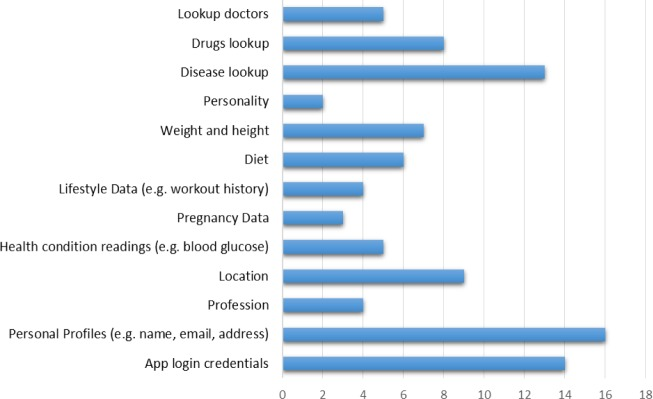
\includegraphics[width=0.95\textwidth]{img/sensitivedistribution.jpg}
  \caption{Sensitive information distribution for study 3 (taken from  He et al. \cite{he2014security})}
  \label{fig:sensitivedistribution}
\end{figure}

% EM QUE O TRABALHO ME AJUDOU
The work by He, Dongjing, et al. \cite{he2014security} helped in understanding what are the most common attack surfaces when considering mHealth applications on Android and it also helped assessing the security risks inherent to applications which handle privacy sensitive information. This paper generally describes the state-of-the-art of security in commercial mobile health apps and pinpoints what should be fixed in order to build better and more secure application for the healthcare industry. It is clear that developers focus much more on building feature-full applications rather than secure applications and this is way it is important to build a framework which allows developers to completely focus on the features they want to provide without having to focus heavily on security. We believe that building a developer framework over ARM's TrustZone technology is a good solution because with TrustZone is possible to fully enjoy the potential of the hardware already available in most mobile devices. This technology will be described in section \ref{sec:trustzone}. 

\subsection{Mobile Security}
%
%TEXT HERE\\
%TEXT HERE\\
%TEXT HERE
%
\subsection{TrustZone}
\label{sec:trustzone}
%
%TEXT HERE\\
%TEXT HERE\\
%TEXT HERE
%
%\subsubsection*{Andix OS\\}
%TEXT HERE\\
%TEXT HERE\\
%TEXT HERE

%% Example citation:
%THIS IS A CITATION\cite{Braem2013a}
%
%The related work section will highly volatile, and will mostly depend on your kind of thesis. Talk with your supervisor in order to know how to write this part. Don't take the following bullet points as a certain truth.
%
%\begin{itemize}
%  \item Most important part of the document. Might be divided in 2/3 subsections.
%  \item Might be devised into related work and 
%  \item Should cite a wide range of references ~30, search in google, google scholar, mendley, IEEE explorer etc..
%  \item Summarized table of solutions.
%\end{itemize}
%
%Citations should be mostly :
%\begin{itemize}
%  \item magazine articles
%  \item conferences / workshops
%  \item books and technical reports
%\end{itemize}
%And make sure that your citations follow the following criteria:
%\begin{itemize}
%  \item Conferences: name and year
%  \item workshops: name of the workshop, name of the conference, location and year
%  \item Magazines: volume, issue (if possible article pages), publisher.
%  \item Books: title, publisher, ISBN, year
%\end{itemize}
%Websites should be added as footnotes~\footnote{www.google.com}
%
% Example image:
%\begin{figure}[hb!]
%  \centering
%  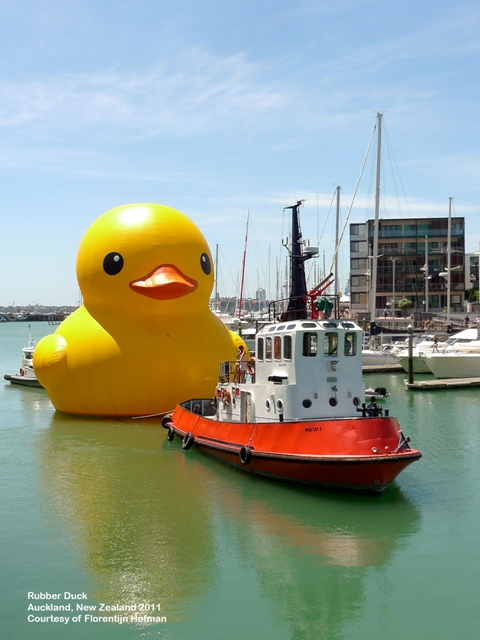
\includegraphics[width=0.95\textwidth]{img/rubberduck.jpg}
%  \caption{caption}
%  \label{fig:label}
%\end{figure}





